In this section, you will describe all of the various artifacts that you will generate and maintain during the project lifecycle. Describe the purpose of each item below, how the content will be generated, where it will be stored, how often it will be updated, etc. 

\subsection{Project Charter}
Generated as a team effort. no need to be maintained as it is a one-time document. Stored in GitHub team repository.

\subsection{Product Backlog}
Generated each sprint cycle with team input. Maintained daily, weekly, each cycle. Stored in Leankit project tracking app.

\subsection{Sprint Planning}
Generated as a team effort at the beginning of each sprint. Maintained daily on the Leankit tracking app.

\subsubsection{Sprint Goal}
Generated at the beginning of each sprint cycle through team input. Progressed maintained daily with workup to final production of the goal. Whether the goal has been achieved is agreed upon by each team member.

\subsubsection{Sprint Backlog}
Generated as a team effort at the beginning of each sprint. Maintained daily on the Leankit tracking app.

\subsubsection{Task Breakdown}
Delegated and agreed upon at the beginning of sprint cycles and team meetings. Tracked through Leankit as well as the online repository.

\subsection{Sprint Burndown Charts}
Generated at end of each sprint cycle. Maintained after each and every cycle. It would be stored on the repository.

\begin{figure}[h!]
    \centering
    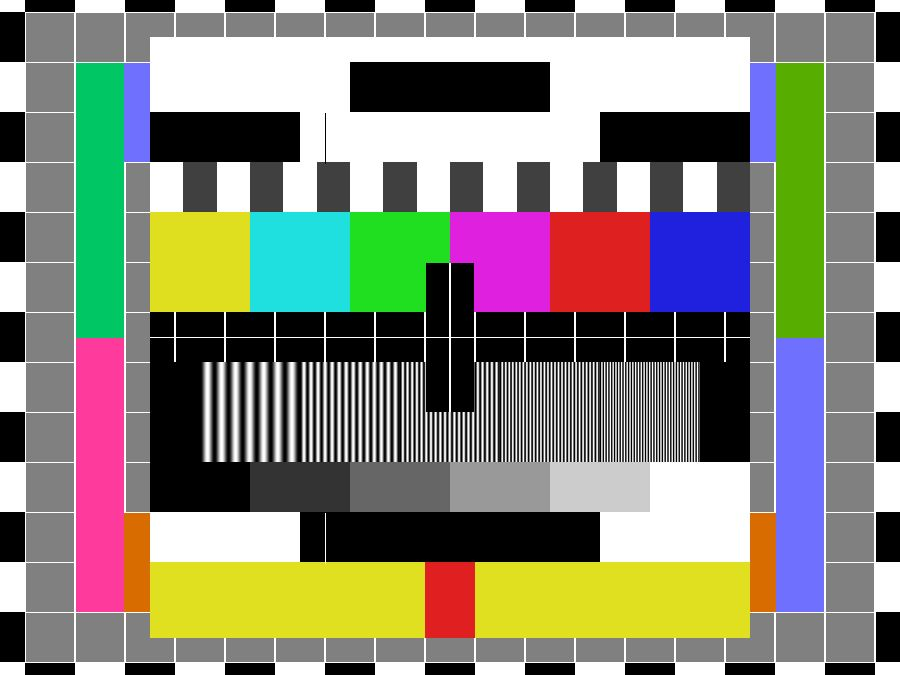
\includegraphics[width=0.5\textwidth]{images/test_image}
    \caption{Example sprint burndown chart}
\end{figure}

\subsection{Sprint Retrospective}
Generated at end of each sprint cycle. Maintained after each and every cycle. It would be stored on the repository.

\subsection{Individual Status Reports}
Done at each and every team meeting and stored in the Github repository.

\subsection{Engineering Notebooks}
Maintained at every thought by each member of the team at their digression.

\subsection{Closeout Materials}
Mechanical designs, code, mockups, protoypes, any documentations used to make the product, the and user manual.

\subsubsection{System Prototype}
mockup before the actual building. Stored in Senior design lab.

\subsubsection{Project Poster}
Generated by the team stored in the senior design lab.

\subsubsection{Web Page}
Made by and for the team.

\subsubsection{Demo Video}
Stored on team webpage made by and for the team.

\subsubsection{Source Code}
All code including test code stored and maintained on team repository.

\subsubsection{Source Code Documentation}
Integrated in code and supporting documentation. Maintained and updated as needed on the repository.

\subsubsection{CAD files}
If generated by team and used for testing purposes, will be stored on team repository and made available on team webpage.

\subsubsection{User Manual}
Created by for about us made available on the webpage and stored on the repository.